\chapter{Testing}
\label{chap:testing} 

Dieses Kapitel beschreibt, wie wir unseren Bot und dessen Komponenten getestet haben. Das Testen beanspruchte einen grossen Teil unserer aufgewendeten Zeit. Die nachfolgenden Methoden zeigen auf, wie wir versuchten m�glichst effizient zu testen, so dass uns mehr Zeit f�r das implementieren der Module blieb. In vielen F�llen machten wir gute Erfahrungen damit, mit gezielten Unit-Tests die Entwicklung des Codes voranzutreiben. Zu behaupten, wir h�tten dabei Test Driven Development (TDD)\footnote{Bei der testgetriebenen Entwicklung erstellt der Programmierer Software-Tests konsequent vor den zu testenden Komponenten. (Def. Wikipedia)} angewandt, w�re �bertrieben, aber bei verschiedenen Modulen orientierten wir uns an den Ideen von TDD, um rasch und zuverl�ssig funktionierende Code zu schreiben.

\section{UnitTests}
\label{sec:testCenter.UnitTests}

Dank dem modularen Aufbau des Java-Codes war es uns gut m�glich, einzelne Module zu testen. F�r unsere UnitTests verwendeten wir die JUnit 4 Library. So findet man in jedem Java Project das Code-Package und ein UnitTest-Package, welches den Code auf dessen Richtigkeit pr�ft. Die Module wurden erst nach den erfolgreichen UnitTests in den Bot eingebaut. Dies hat den Vorteil, dass die Fehlern nicht im laufenden Spiel auftraten und wir die Ursachen  m�hsam suchen mussten.

Beim Combat Positioning\footnote{siehe Kapitel \ref{sec:module.CombatSituation}} haben wir uns am meisten an Test Driven Development orientiert. Wir haben im Test verschiedenste Szenarien eingegeben, die im Kampf auftauchen k�nnten, und haben dann den Code so erweitert, dass f�r diese Szenarien gute L�sungen gefunden wurden. Auf diese Weise sind wir bei der jetzigen Implementierung des Combat Positioning angekommen, die eine ganz gute N�herung an eine optimale Kampfformation darstellt.

\section{Visuelle Tests}
\label{sec:testCenter.VisuelleTests}

In Form eines UnitTest haben wir auch unsere visuellen Tests geschrieben. Eine visuelle �berpr�fung des Resultats ist meistens, vor allem bei der Pfadsuche, einfacher zu kontrollieren. Im Gegensatz zu JUnit wo das zu erwartende Resultat mit Assertions (z.B. \texttt{assertEquals()}) gepr�ft wird, haben die visuellen Test ein HTML-File als Output. In das HTML-File wird die Karte in Tabellenform gespeichert. In jeder Zelle der Tabelle k�nnen Objekte (Einheiten, H�gel, Wegpunkte etc.) durch farbige Punkte dargestellt werden. Diese Funktionalit�ten bietet die extra daf�r geschriebene Klasse MapOutput. Nachfolgend ist ein HTML-File abgebildet mit welchem wir die Korrektheit des Clustering und des HPA* Algorithmus visuell �berpr�ft haben. 

\begin{figure}[H]
\centering
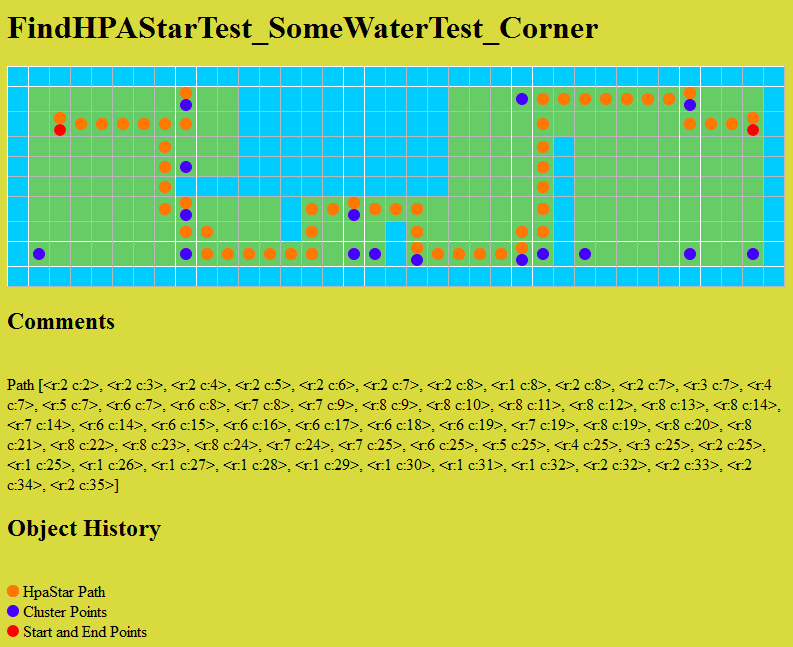
\includegraphics[height=100mm]{91_bilder/mapoutput01}
\caption{HTML-Ausgabe zur visuellen �berpr�fung von HPA*}
\label{fig:mapoutput01}
\end{figure}